\documentclass[a4paper,11pt,openright,oneside]{report}
\usepackage[utf8]{inputenc}
\usepackage[T1]{fontenc}
\usepackage[portuguese]{babel}
\usepackage{graphicx}
\usepackage[backend=biber, style=ieee]{biblatex}
\usepackage{csquotes}
\usepackage{blindtext}
\usepackage[printonlyused]{acronym}
\usepackage{hyperref}
\usepackage{minted}
\usepackage[titletoc,title]{appendix}

\newcommand{\RNum}[1]{\uppercase\expandafter{\romannumeral #1\relax}}

\bibliography{Crypto.bib}

\begin{document}

\begin{titlepage}
\begin{center}

{\vspace*{50mm}\textsc{\Huge\textbf{Criptografia}\\ \small{Laboratórios de Informática}}}\\[2cm]
{\textsc{\small\textbf{Universidade de Aveiro}}}\\[0.5cm]
{\small Nelson Costa 42983\\Ricardo Jesus 76613}\\[0.5cm]
{\small	15 de Março de 2015}\\

\begin{figure}[b]
\center
\graphicspath{}

\includegraphics[height=2cm]{ua.pdf}
\end{figure}

\end{center}

\end{titlepage}

\title{\textbf{Criptografia}\\[1cm]\textsc{\small {Departamento de Electrónica, Telecomunicações e Informática} \\ \large {UNIVERSIDADE DE AVEIRO}}}
\author{Nelson Costa 42983, Ricardo Jesus 76613\\nelson.costa@ua.pt, ricardojesus@ua.pt}
\date{15 de Março de 2015}

\maketitle

\pagenumbering{roman}

\begin{abstract}

Com o objetivo de implementar dois programas, um que cifre e outro que decifre um dado ficheiro segundo um esquema híbrido, de forma a fornecer autenticidade e confidencialidade, mantendo ainda assim um rápido processamento do ficheiro, começou por se estudar o que é criptografia simétrica, assimétrica, e de que forma ambas se relacionam de forma a obter um esquema híbrido. De seguida, procedeu-se à implementação dos programas em Python e descreveu-se como foram implementadas as funções que processam a componente criptográfica dos mesmos.

\end{abstract}

\tableofcontents
%\listoftables
\listoffigures

\clearpage
\pagenumbering{arabic}

\chapter{Introdução}
\label{chap.introdução}

Cada vez mais a criptografia desempenha um processo fundamental na sociedade atual. Veja-se como a decifragem de 'Enigma'\footnote{\url{http://en.wikipedia.org/wiki/Enigma_machine}} teve uma tão grande importância no desenrolar da Segunda Guerra Mundial, ou como o recente ataque à 'Sony Pictures Entertainment' fez os Estados Unidos da América temer pela sua cibersegurança.

Assim, e visto que a cada dia que passa estamos mais ligados uns aos outros através, por exemplo, da Web, é cada vez mais necessário manter a confidencialidade na partilha de informação, onde algoritmos de cifragem e decifragem desempenham um processo crucial. Felizmente, nos dias que correm temos à nossa disposição inúmeros algoritmos deste tipo, de onde se destacam os algoritmos simétricos e assimétricos.\\

Em relação aos algoritmos simétricos, destaca-se a velocidade com que determinada informação pode ser cifrada e decifrada. Nestes algoritmos é utilizada uma chave partilhada entre emissor e recetor para transmitir informação de uma forma confidencial. Já em relação a algoritmos assimétricos, estes são centenas senão milhares de vezes mais lentos que os métodos simétricos, no entanto visto utilizarem pares de chaves de forma a garantir transmissão de informação de uma forma segura, onde existe uma chave pública partilhada com os demais e uma privada a que apenas o próprio indivíduo deve ter acesso, este método garante, por exemplo, que um ficheiro cifrado com a chave pública de um indivíduo \textbf{A} pode apenas ser decifrado pelo próprio \textbf{A} com a sua chave privada (note-se que a informação cifrada com uma chave pública só pode ser decifrada pela respetiva chave privada, ou vice-versa). Para além disso, estes métodos por pares de chaves são considerados mais seguros e permitem também dar resposta a questões de autenticidade.\\

Com base nestas vantagens e desvantagens de um e outro métodos, surgiram esquemas de encriptação híbrida que procuram tirar partido das vantagens de ambos os métodos (velocidade da encriptação simétrica e segurança da encriptação assimétrica).

Estes temas relacionados com diferentes formas de cifragem encontram-se desenvolvidos na secção \ref{chap.criptografia} deste relatório.\\

Com isto em mente foram implementados dois programas escritos em linguagem Python e recorrendo à biblioteca PyCrypto. Um funcionando como programa que cifra, e outro que decifra implementando um esquema de encriptação híbrida garantindo a transmissão de informação de forma eficiente e segura. A análise recorrente da implementação destes programas encontra-se na secção \ref{chap.programas}.

\chapter{Criptografia}
\label{chap.criptografia}

A criptografia é a arte ou ciência de escrever uma mensagem de forma a ocultar o seu conteúdo. Dito por outras palavras, a criptografia usa técnicas que permitem que várias entidades possam transmitir mensagens de forma segura e privada, sem que estas sejam intercetadas e aproveitadas por terceiros. Independentemente do método que for usado para ocultar dados, a criptografia moderna pretende satisfazer quatro objetivos fundamentais:

\begin{description}
\item[Confidencialidade:] caso alguém intercete uma mensagem, essa pessoa não deve ser capaz de ler e perceber o seu conteúdo.
\item[Integridade dos dados:] o destinatário da mensagem deve ser capaz de verificar se a mensagem foi alterada durante a transmissão, acidental ou deliberadamente.
\item[Autenticação:] o destinatário da mensagem deve ser capaz de verificar a sua origem.
\item[Não-repúdio:] o remetente não deve ser capaz de negar mais tarde que foi quem realmente enviou a mensagem para o destinatário.
%O destinatário também não deve ser capaz de negar que recebeu a respetiva mensagem.
\end{description}

Existem alguns conceitos que são essenciais para a compreensão das operações envolvidas em criptografia. O termo \textbf{cifra} é o processo que transforma um texto em claro num texto cifrado, ou também designado por criptograma. O termo \textbf{decifra} é a operação inversa da cifra, ou seja, transforma o criptograma no texto em claro original. As operações de cifra e decifra usam algoritmos e chaves, sendo estas utilizadas como parâmetros nos ditos algoritmos. Os algoritmos são modelos matemáticos que contêm um conjunto de operações (ou regras) que permitem transformar os dados, ou seja, neste contexto possibilitam as operações de cifra e decifra. A figura \ref{fig:crypto0} mostra os processos básicos de cifragem e decifragem na criptografia.

\begin{figure}[ht]
\center
\fbox{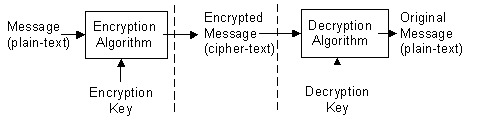
\includegraphics[height=3cm]{crypto0.jpg}}
\caption{Processos básicos de cifragem e decifragem na criptografia.}
\label{fig:crypto0}
\end{figure}

A mensagem original (\textit{plain-text}) é cifrada usando um algoritmo e uma chave, produzindo uma mensagem cifrada (\textit{cipher-text}). A mensagem cifrada é por sua vez decifrada usando outro algoritmo e outra chave (que até poderá ser igual à usada no processo de cifragem), obtendo-se a mensagem original (\textit{plain-text}).\\

A criptografia pode ser dividida em várias áreas, entre as quais as funções de síntese e as criptografias simétrica, assimétrica e híbrida.

\section{Funções de Síntese}

Existem três tipos de algoritmos criptográficos: os com chaves simétricas, assimétricas e as funções de síntese (\textit{Digest functions} ou \textit{Hash functions}). Ao contrário dos que utilizam chaves, as funções de síntese apenas processam um determinado ficheiro, sem necessitarem de qualquer chave. Estas funções produzem um valor de dimensão constante (\textit{hash value}) a partir de um volume arbitrário de bits. Além disso, devem garantir a obtenção de valores diferentes mesmo para ficheiros semelhantes (se bem que é extremamente dificil garantir a não ocorrência de colisões). O principal objetivo destas funções na criptografia é a integridade dos dados. O valor que é produzido fornece uma impressão digital (\textit{digital fingerprint}) do conteúdo da mensagem, o que permite assegurar que caso a mensagem for alterada por pessoas mal-intencionadas ou, por exemplo, vírus, isso não passa despercebido. São vários os algoritmos que produzem estas sínteses, entre os quais o MD5 e o SHA-1 com 128 e 160 bits de tamanho, respetivamente. Estes algoritmos podem ser considerados mais ou menos eficientes em função da facilidade com que se consegue obter um mesmo valor de hash para ficheiros diferentes.\\

Uma das situações onde se podem encontrar as funções de síntese é nas assinaturas digitais. A figura \ref{fig:crypto5} esquematiza de forma simples os processos associados à produção de documentos assinados digitalmente.

\begin{figure}[ht]
\center
\fbox{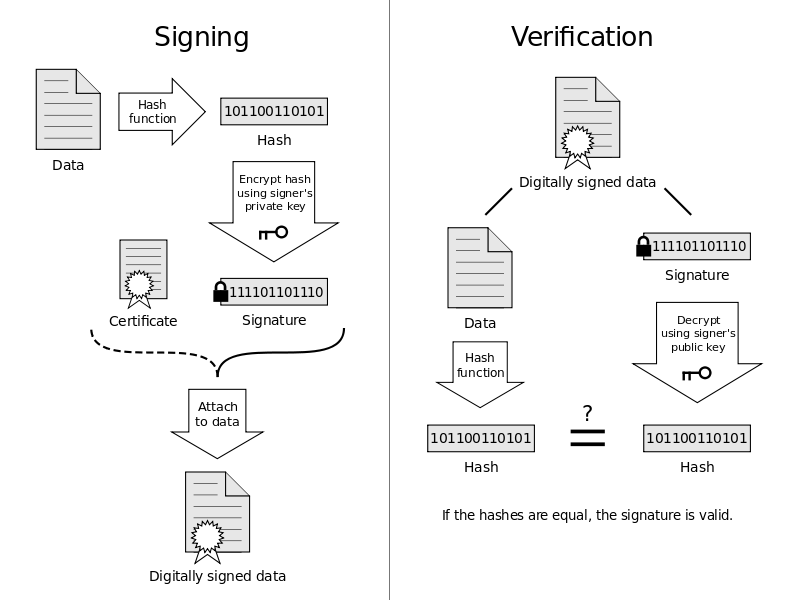
\includegraphics[height=8cm]{crypto5.png}}
\caption{Criação de assinaturas digitais com funções de síntese.}
\label{fig:crypto5}
\end{figure}

O remetente da mensagem cria uma assinatura digital aplicando uma função de síntese (\textit{Hash function}) no documento (\textit{Data}), produzindo-se um ficheiro sintetizado (\textit{Hash}). Este ficheiro é cifrado usando a chave privada do emissor de forma a produzir uma assinatura digital que é depois anexada ao documento (\textit{Digitally signed data}). Após a receção do documento assinado, o destinatário decifra a assinatura através da chave pública do assinante e executa uma síntese ao próprio ficheiro. São produzidos dois valores 'hash' e ambos comparados, i.e., se forem iguais a assinatura é considerada válida.\\

De referir que no contexto das assinaturas digitais são aplicados dois objetivos da criptografia moderna: o do não-repúdio e garatia de integridade de dados. Ou seja, o remetente não deverá ser capaz de negar mais tarde que foi realmente a pessoa que enviou a mensagem, e o recetor deverá ser capaz de verificar, para além da origem da mesma, que esta se encontra no mesmo estado em que foi enviada.

\section{Criptografia Simétrica}
\label{chalp.simétrica}

A cifra simétrica é a forma mais básica de criptografia na qual é partilhada uma chave entre o emissor e o recetor da mensagem, geralmente designada por chave simétrica, e usada por ambos para cifrar e decifrar mensagens. Além de possuírem a mesma chave, os intervenientes também devem possuir o mesmo algoritmo, neste caso designado por algoritmo simétrico. A figura \ref{fig:crypto1} ilustra de forma simples o uso de chaves partilhadas na criptografia simétrica.

\begin{figure}[ht]
\center
\fbox{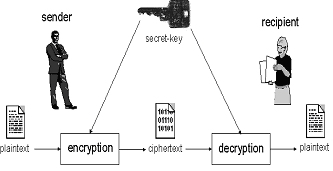
\includegraphics[height=4cm]{crypto1.jpg}}
\caption{Uso de chave partilhada na criptografia simétrica.}
\label{fig:crypto1}
\end{figure}

O remetente (\textit{sender}) cifra o texto em claro (\textit{plaintext}) através da chave simétrica (\textit{secret-key}), produzindo-se um texto cifrado (\textit{ciphertext}). O destinatário (\textit{recipient}) da mensagem decifra-a usando a chave partilhada por ambos. O processo contrário também se pode realizar, ou seja, a chave tanto pode servir para cifrar como para decifrar mensagens.\\

A criptografia simétrica divide-se em dois tipos de cifras: a contínua e a por blocos.

\subsection{Cifras Simétricas Contínuas}

Na cifra contínua, a mensagem em claro é tratada como uma sequência de bytes (ou bits) onde cada sequência é cifrada sequencialmente. Usa uma operação relativamente simples para misturar a mensagem original com uma chave contínua pseudo-aleatória de dimensão finita também designada por \textit{keystream}. Esta operação é tipicamente a função XOR (Exclusive-OR)\footnote{\url{http://en.wikipedia.org/wiki/Exclusive_or}} visto que é uma função facilmente invertível.\\

A operação de cifra consiste em aplicar a função XOR entre a mensagem a transmitir e a chave utilizada na operação. A expressão \ref{eq1} mostra como é feita a operação de cifra.

\begin{equation}
\label{eq1}
C = T \oplus Ks
\end{equation}

Onde C é o criptograma, T é o texto em claro e Ks a chave contínua (\textit{keystream}).\\

A operação de decifra pode ser executada aplicando novamente a função XOR. A expressão \ref{eq2} mostra como é feita a operação de decifra.

\begin{equation}
\label{eq2}
T = C \oplus Ks
\end{equation}

Onde T é o texto em claro, C é o criptograma e Ks a chave contínua (\textit{keystream}).\\

De referir que é usada a mesma chave nas duas equações (\ref{eq1} e \ref{eq2}).

\subsection{Cifras Simétricas por Blocos}

Na cifra por blocos, a mensagem é dividida em blocos de igual dimensão sendo cada um deles processados de forma independente dos restantes (se bem que podem existir mecanismos de feedback). Conforme o algoritmo aplicado para cifrar e decifrar mensagens, os blocos podem ter dimensões diferentes. Por exemplo, o DES (\textit{Data Encryption Standard}) e o AES (\textit{Data Encryption Standard}) são dois algoritmos bastante usados neste tipo de cifra, mas em que ambos utilizam blocos de tamanhos distintos, 64 e 128 bits respetivamente. O criptograma é criado após a criação de vários pequenos criptogramas representando cada um dos blocos cifrados.\\

Um conceito bastante importante neste tipo de cifra é o alinhamento, ou \textit{padding}. Existem modos de cifra por blocos que põem particularmente em prática este conceito. Um deles é o ECB (\textit{Electronic Code Book}), que possibilita a separação de ficheiros em blocos de dimensões iguais. Por exemplo, se um determinado ficheiro for separado em blocos e verificar-se que o último não tem uma dimensão igual à dos restantes, é adicionado uma “string” de bytes (ou bits) no final desse bloco de forma a obter o tamanho pretendido. Esse acréscimo de bits forma um excipiente, sendo importante indicar a sua existência e comprimento de forma a facilitar a decifra por parte de quem recebe a mensagem cifrada. A figura \ref{fig:crypto2} ilustra muito basicamente os processos de cifragem nas cifras contínuas e por blocos.

\begin{figure}[ht]
\center
\fbox{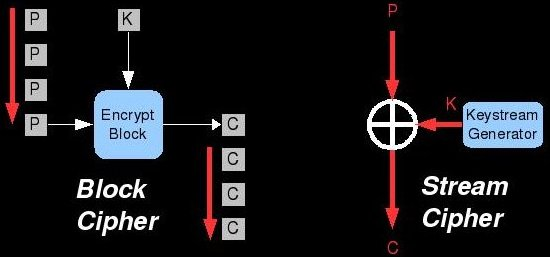
\includegraphics[height=5cm]{crypto2.jpg}}
\caption{Processos de cifragem na cifra por blocos (\textit{Block Cipher}) e contínua (\textit{Stream Cipher}).}
\label{fig:crypto2}
\end{figure}

Na cifra por blocos, o texto em claro é 'partido' em blocos de dimensões iguais (P1, P2, …, Pn) sendo cada um deles cifrados de forma independente dos restantes, obtendo-se vários criptogramas (C1, C2, …, Cn) que todos juntos formam o criptograma principal. Na cifra contínua, é gerada uma chave contínua e combinando-a com o texto em claro com a função XOR gera-se o criptograma (C).

\section{Criptografia Assimétrica}
\label{chap.assimétrica}

A criptografia assimétrica é uma área da criptografia onde cada um dos interlocutores possui um par de chaves, uma privada (ou secreta) e outra pública. A chave pública é usada principalmente para cifrar mensagens ou para verificar assinaturas digitais. O termo \textbf{assimétrico} vem do facto de se usarem duas chaves, mas ambas com funções opostas. A criptografia assimétrica usa cifras por blocos e pode assegurar a confidencialidade e a autenticação nas mensagens transmitidas dependendo de como se usam as chaves.\\

Se se pretender comunicar confidencialmente, a chave pública do destinatário é usada para cifrar e a chave privada do destinatário é usada para decifrar, ou seja só o destinatário conseguirá decifrar o criptograma através da sua chave privada. Por outro lado, o destinatário não tem conhecimento de quem remeteu a mensagem cifrada (pelo menos isso não pode ser garantido), e sendo assim a autenticação não pode ser verificada. A figura \ref{fig:crypto3} ilustra o uso correto das chaves assimétricas para garantir a confidencialidade na transmissão das mensagens entre emissor e recetor.

\begin{figure}[ht]
\center
\fbox{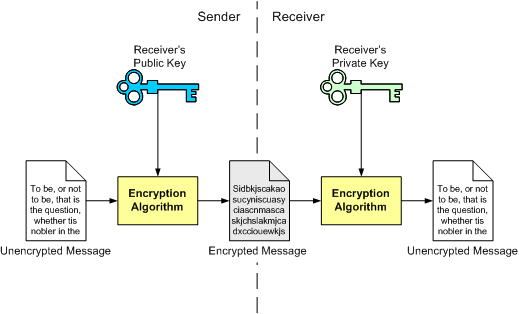
\includegraphics[height=6cm]{crypto3.png}}
\caption{Criptografia assimétrica e confidencialidade.}
\label{fig:crypto3}
\end{figure}

O remetente (\textit{sender}) deve conhecer a chave pública do destinatário (\textit{receiver}) para cifrar as suas mensagens e assim comunicar de forma confidencial. O destinatário usa por sua vez a sua chave privada para decifrar o criptograma. Neste caso, só é usado o par de chaves do lado do destinatário.\\

Por outro lado, se o remetente pretender garantir a autenticação da origem da mensagem recebida, por exemplo na transmissão de documentos com assinaturas digitais, as chaves são usadas de forma contrária, ou seja, a chave privada do remetente é usada para cifrar as mensagens e a sua chave pública usada para as decifrar. O destinatário decifra o criptograma usando a chave pública do remetente e verifica que foi este último quem gerou o criptograma. Neste caso não há confidencialidade visto que a chave usada para decifrar é pública (chave pública do remetente), ou seja, quem a conhecer poderá decifrar o criptograma. A figura \ref{fig:crypto4} ilustra a transmissão de mensagens usando chaves assimétricas para garantir a autenticação da origem das mesmas.\\

\begin{figure}[ht]
\center
\fbox{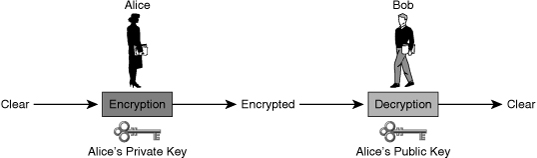
\includegraphics[height=3cm]{crypto4.jpg}}
\caption{Criptografia assimétrica e autenticação.}
\label{fig:crypto4}
\end{figure}

O emissor (\textit{Alice}) cifra a mensagem através de um algoritmo assimétrico e da sua chave privada (\textit{Alice’s Private Key}) e envia para o destinatário (\textit{Bob}) o criptograma gerado. Este, por sua vez, decifra-o através da chave pública do emissor (\textit{Alice’s Public Key}) verificando a autenticação do autor. Neste caso, só se usa o par de chaves do lado do emissor.\\

Um dos algoritmos mais utilizados neste método é o RSA\footnote{\url{http://en.wikipedia.org/wiki/RSA_(cryptosystem)}} que tira partido de certas propriedades de números primos e da dificuldade e exigência de recursos necessários para factorizar grandes inteiros.

\section{Criptografia Híbrida}
\label{chap.híbrida}

A cifragem híbrida tira partido não só da segurança extra e autenticidade que algoritmos assimétricos permitem, como também da velocidade oferecida por algoritmos simétricos. Assim, este método procura juntar o melhor de ambos os processos. O que geralmente é permitido é a cifragem da mensagem a transmitir, que poderá ser um ficheiro bastante grande e onde, portanto, torna-se muito mais proveitoso utilizar um algoritmo simétrico segundo um método de cifragem simétrica. No entanto, a chave utilizada para cifrar o ficheiro é (geralmente) gerada aleatoriamente, sendo guardada noutro ficheiro e cifrada segundo um processo de chaves assimétricas. Quando o ficheiro principal é enviado, juntamente envia-se a chave simétrica utilizada para o cifrar por exemplo num ficheiro auxiliar (relembre-se que esta chave simétrica encontra-se também ela cifrada).\\

Veja-se um simples exemplo de utilização, em que um certo indivíduo \textbf{A} pretende enviar uma mensagem cifrada a outro \textbf{B}, segundo este esquema de cifragem híbrida:

\begin{enumerate}
\item \textbf{A} terá de obter a chave pública de \textbf{B}.
\item Gera-se uma chave simétrica aleatória.
\item Cifra-se a mensagem segundo um algoritmo de cifragem simétrica como AES.
\item A chave simétrica utilizada é cifrada segundo um algoritmo assimétrico (utilizando a chave pública de \textbf{B})
\item Ambas a mensagem e a chave cifradas são enviadas a \textbf{B}.
\end{enumerate}

O que \textbf{B} terá de fazer quando receber os ficheiros, de forma a decifrar a mensagem, deverá ser algo como:

\begin{enumerate}
\item \textbf{B} utiliza a sua chave privada para decifrar a chave simétrica utilizada para cifragem da mensagem.
\item É utilizada essa chave simétrica para decifrar a mensagem enviada.
\end{enumerate}

\chapter{Implementação de Programas}
\label{chap.programas}

Neste capítulo irá ser abordada a implementação de dois programas, um com o objetivo de cifrar e o outro de decifrar uma certa mensagem. Ambos utilizam um esquema híbrido (\ref{chap.híbrida}), portanto fornecendo confidencialidade e autenticidade mas permitindo uma rápida cifragem e decifragem da mensagem a ser enviada. Os pares de chaves assimétricas utilizados nos testes destes programas foram gerados utilizando o programa \href{run:../Python/KeysGenerator/generateKeys.py}{\textbf{generateKeys.py}}. O código de ambos os programas para além de ser enviado em anexo é também disponibilizado (em anexo) no final deste relatório para facilitar o confronto do código face à análise levada a cabo sobre ele em cada uma das secções seguintes, secções onde se procura explicar como se resolveu o problema inicialmente exposto.

Os programas foram escritos na linguagem de programação \verb|Python (2.7)|, e recorreu-se extensamente à biblioteca \verb|PyCrypto|\footnote{\url{https://www.dlitz.net/software/pycrypto/}} para implementar os processos relacionados com cifragem e decifragem de informação.\\


Visto estar a ser utilizado um esquema de encriptação híbrida, o ficheiro principal a transmitir é cifrado recorrendo-se a um algoritmo com chaves partilhadas, neste caso AES. Na utilização deste algoritmo, escolheu-se o modo de operação CFB, que é um método de encriptação contínua auto-sincronizada (\textit{self-synchronizing stream encryption}), garantindo assim que a geração do criptograma não é feita apenas pela aplicação do operador XOR entre a mensagem e uma chave, mas em que há uma relação de feedback entre o criptograma a ser gerado e o resto do criptograma a gerar (um pouco como cifras por blocos). Isto juntamente com a existência de um valor 	\verb|iv| (\textit{initialization vector}) que serve como fator aleatório extra neste processo de feedback, garante que um mesmo ficheiro que seja cifrado várias vezes com uma mesma chave dará origem a criptogramas diferentes e portanto é mais difícil desvendar o que se está a transmitir. Um exemplo da implementação deste algoritmo é visível nas figuras \ref{fig:crypto6} e \ref{fig:crypto7}.

\begin{figure}[ht]
\center
\fbox{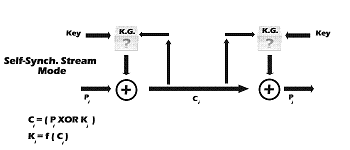
\includegraphics[height=3cm]{crypto6.png}}
\caption{Cifragem com AES modo CFB}
\label{fig:crypto6}
\end{figure}

\begin{figure}[ht]
\center
\fbox{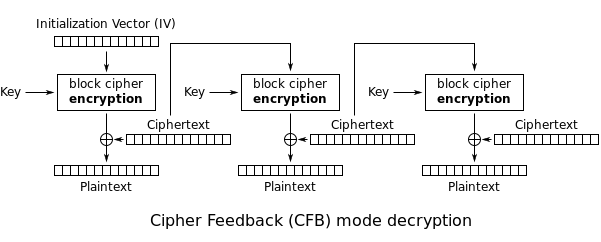
\includegraphics[height=3cm]{crypto7.png}}
\caption{Decifragem com AES modo CFB}
\label{fig:crypto7}
\end{figure}

No entanto, devido à forma como é processado este aumento de segurança também acarreta um decréscimo na velocidade de cifragem e decifragem. Apesar disso escolheu-se usá-lo já que se o maior fator de interesse nestes programas fosse meramente a velocidade, então não se estaria sequer a seguir um esquema híbrido.\\

Para facilitar certas explicações abaixo, parte-se do princípio de que o indivíduo \textbf{A} quer enviar um ficheiro cifrado a \textbf{B}, que só este último pode decifrar, e em que é possível verificar a autenticidade do ficheiro.

\section{Cifragem}

O programa responsável pela cifragem da mensagem a transmitir é \href{run:../Python/Sender/encipher.py}{\textbf{encipher.py}}. O código do programa é incluido neste relatório em \ref{App:encipher.py}.
Este programa depende de várias funções para sua execução, destancando-se as \verb|sigGenerator|, \verb|keyGenerator| e \verb|encipher|. Outras funções nele presentes estão relacionadas com a robustez do programa e não com a cifragem da mensagem em si, e portanto não irão ser abordadas.\\

O objectivo deste programa é tirar partido da velocidade de algoritmos de cifragem com chaves simétricas, mas manter as funcionalidades e segurança extra que os com chaves assimétricas permitem. Com isso em mente, é gerada uma chave simétrica pelo programa, que é cifrada com a chave pública de \textbf{B} (para que apenas este a possa decifrar), a assinatura do ficheiro é cifrada com a chave privada de \textbf{A} (para que \textbf{B} possa ter certezas sobre a origem do ficheiro e se foi adulterado ou não), e o ficheiro em si é cifrado com a chave simétrica gerada, sendo portanto muito mais rápida a sua cifragem e decifragem.\\

Apesar de nas funções a seguir expostas se falar na criação de ficheiros auxiliares (\verb|*.sig| e \verb|*.key|) e dum ficheiro principal \verb|*.bin|, estes não estão presentes no final da execução do programa já que se optou por juntar todos estes ficheiros num único \verb|*.all|, facilitando assim o envio do ficheiro cifrado. Este processo é um dos implementados pelas funções auxiliares referidas acima, não estando relacionado com a cifragem em si.

\subsection{sigGenerator}

Esta função é responsável pela criação de uma assinatura do ficheiro, de forma a garantir ao recetor da mensagem que o que ele está a receber (e irá decifrar) é de facto a mensagem enviada (ou, no caso de não ser, pelo menos isso será facilmente verificado). Para além disso, o recetor saberá também com certeza que a mensagem foi enviada pelo indivíduo \textbf{A}.\\

Para isto recorre-se a uma função de síntese, \verb|SHA-256|\footnote{\url{http://en.wikipedia.org/wiki/SHA-2}}, para calcular a \verb|hash| do ficheiro a cifrar. De seguida recorre-se ao módulo \verb|PKCS1_v1_5|\footnote{\url{https://www.dlitz.net/software/pycrypto/api/current/toc-Crypto.Signature.PKCS1_v1_5-module.html}} para gerar a assinatura do ficheiro com a chave privada de \textbf{A} e este \verb|hash|, sendo esta gravada num ficheiro \verb|*.sig|, onde \verb|*| simboliza o nome do ficheiro original sem extensão.

\subsection{keyGenerator}

Esta função tem como objectivo gerar e guardar a chave simétrica usada pelo programa, cifrando-a com a chave pública de \textbf{B} (de forma a que apenas este a possa decifrar). Para isso, inicialmente gera-se uma sequência aleatória de 1024 bits. Visto que o método de encriptação AES necessita de chaves com 16, 24 ou 32 bytes, é calculada a síntese \verb|SHA-256| do código aleatório gerado de forma a garantir que a chave final é de 256 bits (ou seja, 32 bytes). De seguida esta chave é cifrada com a chave pública de \textbf{B} recorrendo-se ao módulo \verb|PKCS1_OAEP|\footnote{\url{https://www.dlitz.net/software/pycrypto/api/current/toc-Crypto.Cipher.PKCS1_OAEP-module.html}}, garantindo-se assim que apenas \textbf{B} pode decifrar esta chave (com a sua chave privada), obtendo a chave necessária à decifragem da mensagem enviada. O resultado é depois guardado num ficheiro \verb|*.key|, onde mais uma vez \verb|*| simboliza o nome do ficheiro a cifrar sem extensão.\\

Para além da chave cifrada, é também guardado um código \verb|iv| (\textit{initialization vector}) necessário à correta descodificação da mensagem. Este código é gerado na função \verb|encipher|, sendo que a função \verb|keyGenerator| apenas o guarda no mesmo ficheiro onde a chave é guardada. Este código é necessário em resultado da utilização do modo de encriptação de AES CFB\footnote{\url{http://goo.gl/RxmaQC}}.

\subsection{encipher}

Por último, processa-se de facto a cifragem do ficheiro recorrendo-se para isso à função \verb|encipher|. Esta recorre às duas funções anteriormente expostas de forma a obter os resultados nelas expostos, gera também um código de 16 bytes chamado de \verb|iv|\footnote{\url{http://en.wikipedia.org/wiki/Initialization_vector}} e necessário pelo modo de cifragem em uso, e finalmente cifra o ficheiro original recorrendo ao módulo de cifragem AES\footnote{\url{https://www.dlitz.net/software/pycrypto/api/current/toc-Crypto.Cipher.AES-module.html}}, modo CFB (\textit{Cipher FeedBack}), sendo o resultado guardado num ficheiro \verb|*.bin|.\\

O recetor da mensagem, indivíduo \textbf{B}, poderá utilizar a sua chave privada para obter a chave simétrica gerada para cifrar este ficheiro e poderá utilizar a chave pública de \textbf{A} para garantir a sua origem. Desta forma tira-se partido da velocidade de cifragem com chaves simétricas, mas mantém-se a segurança extra (e autenticação) que chaves assimétricas permitem.

\section{Decifragem}

A decifragem da mensagem cifrada enviada é feita pelo programa \href{../Python/Receiver/decipher.py}{\textbf{de\-ci\-pher.py}} também disponível em \ref{App:decipher.py}. Também este recorre essencialmente a três funções para decifrar o ficheiro recebido, possuindo no entanto mais código responsável por aumentar a sua robustez e utilidade. O seu principal ojectivo é ser capaz de decifrar a chave simétrica utilizada inicialmente para cifrar a mensagem (com a chave privada do utilizador do programa decifrador, ou seja, com a chave privada do indivíduo \textbf{B}), e com ela decifrar a mensagem inicial. Posto isto, é corrida uma função de verificação que visa garantir não só a integridade do ficheiro como também a sua autenticidade. Para isto, o ficheiro onde foi guardada a assinatura do ficheiro original é decifrado com a chave pública de \textbf{A} (quem envia a mensagem), sendo depois analisada a integridade do ficheiro comparando a sua síntese \verb|SHA-256| com a originalmente guardada. De seguida irão ser analisadas em maior detalhe cada uma das funções relacionadas com a decifragem do ficheiro.

\subsection{sigVerification}

Esta é a função encarregue de verificar a autenticidade e integridade do ficheiro recebido. É de notar que mesmo que a verificação falhe a decifragem prossegue.\\

Para garantir a autenticidade e integridade do ficheiro, quando este foi cifrado foi gerada uma assinatura, guardada num ficheiro auxiliar \verb|*.sig|. Desta forma, é agora possível ao utilizador \textbf{B}, por meio do programa \verb|decipher.py|, inferir sobre a origem da mensagem recebida bem como se foi ou não adulterada. Para isto, recorre-se novamente ao módulo \verb|PKCS1_v1_5|, em especial à sua função \verb|RSASSA-PKCS1-V1_5-VERIFY|\footnote{\url{http://goo.gl/OPdiHU}} que permite, tal como o nome indica, correr as verificações pretendidas.\\

Caso a verificação seja concluída com sucesso será imprimida uma mensagem para o terminal de forma a indicar isso mesmo, acompanhada da síntese \verb|SHA-256| do ficheiro. Caso contrário, apenas surgirá uma mensagem indicando que a verificação falhou.

\subsection{keyReader}

Esta função é a que permite a obtenção da chave (de 32 bytes) usada aquando da cifragem simétrica, bem como do código \verb|iv| (de 16 bytes) utilizado no mesmo processo. Ambas as chaves encontram-se guardadas no ficheiro \verb|*.key|, sendo que a chave de 32 bytes está cifrada com a chave pública do recetor (utilizador \textbf{B}) enquanto que o código de 16 bytes não. De forma a obter ambas estas chaves, o programa lê os primeiros 16 bytes do ficheiro \verb|*.key|, onde o código \verb|iv| foi guardado, procedendo-se depois à leitura do resto do ficheiro. Este 'resto' é depois decifrado com a chave privada de \textbf{B} (recorrendo a \verb|PKCS1_OAEP|), obtendo-se assim a chave simétrica utilizada para cifragem do ficheiro original.

\subsection{decipher}

Esta é a função que permite a verdadeira decifragem do ficheiro (no entanto pelo menos a função \verb|keyReader| é também essencial para que esta decifragem seja possível). Esta decifragem é feita de modo inverso à cifragem feita pela função homóloga \verb|encipher| (do programa de cifragem), e, sendo assim, recorre-se também ao algoritmo AES, modo CFB, com o mesmo valor \verb|iv| para decifragem do ficheiro. A chave utilizada nesta decifragem é também a mesma para a cifragem (já que estamos perante um algoritmo de cifragem com chaves simétricas), e obtida recorrendo-se à função \verb|keyReader|. No final da decifragem, é levada a cabo a verificação do ficheiro final através da função \verb|sigVerification|.\\

No final, o ficheiro decifrado é guardado num ficheiro com o mesmo nome que o indicado para decifragem, sem extensão.

\chapter{Conclusões}
\label{chap.conclusões}

Foi-nos possível verificar que ao adotar um esquema híbrido podemos tirar partido da velocidade que um método de encriptação com chaves partilhadas permite, bem como por exemplo da segurança extra e autenticação que métodos com pares de chaves oferecem. Posto isto, pudemos implementar dois programas, um que cifra e outro que decifra, que utilizam este mesmo conceito para garantir a transmissão de informação de forma confidencial e de onde se possa inferir sobre a sua autenticidade e integridade. Isto é possível pois recorre-se a um algoritmo simétrico para cifrar (e decifrar) o ficheiro a transmitir (o que poderia não ser viável caso se se recorresse a um método assimétrico visto este ser muito mais lento e enventualmente o ficheiro poder ser de muito grandes dimensões), mas ainda assim sendo a chave simétrica usada neste processo de cifragem ela própria cifrada com a chave pública do receptor (que a decifra com a sua chave privada), e sendo gerada uma assinatura do ficheiro a partir de uma sua síntese e da chave privada do emissor, não se perdem as vantagens de um método de encriptação assimétrica. Isto garante que apenas o recetor será capaz de decifrar a chave que permite decifrar a informação enviada, bem como que este será capaz de verificar o ficheiro recorrendo à sua assinatura, podendo ter certezas sobre a sua origem e se foi ou não adulterado.

Assim sendo, pudemos verificar que nem métodos simétricos nem assimétricos são perfeitos na transmissão de informação de forma segura. No entanto, apesar dos seus possíveis problemas, ambos têm importantes vantagens e desta forma um método de encriptação que se baseie num esquema híbrido poderá ser um bom compromisso entre as qualidades e desvantagens de um, e as qualidades e desvantagens de outro. 

\newpage
%\appendix

\begin{appendices}
\section{encipher.py}
\label{App:encipher.py}

\begin{minted}[frame=lines,fontsize=\footnotesize,linenos]{python}
import os
import sys
import zipfile
from Crypto import Random
from Crypto.Cipher import AES, PKCS1_OAEP
from Crypto.Hash import SHA256
from Crypto.PublicKey import RSA
from Crypto.Random import random
from Crypto.Signature import PKCS1_v1_5


# Define public and private key names for faster usage

# Sender's private key:
priKey = "A_PrivateKey.pem"
# Receiver's public key:
pubKey = "B_PublicKey.pem"

# File name to encrypt
f_name = ""

# Private key password:
priPass = ""


def usage():
    print "python encipher.py <file_name>"
    sys.exit(-1)


def sigGenerator(priKey_fname, f_name, priPass):
    # Opening and reading file to encrypt

    f = open(f_name, "r")
    buffer = f.read()
    f.close()

    # Creating hash of the file. Using SHA-256 (SHA-512 rose problems)

    h = SHA256.new(buffer)

    # Reading private key to sign file with

    keyPair = RSA.importKey(open(priKey_fname, "r").read(), passphrase=priPass)
    keySigner = PKCS1_v1_5.new(keyPair)

    # Saving signature to *.sig file

    f = open(f_name.split('.')[0] + ".sig", "w")
    f.write(keySigner.sign(h))
    f.close()


def keyGenerator(pubKey_fname, f_name, iv):
    # Generating 1024 random bits, and creating SHA-256 (for 32 bits compatibility with AES)

    h = SHA256.new(str(random.getrandbits(1024)))

    # Reading public key to encrypt AES key with

    keyPair = RSA.importKey(open(pubKey_fname, "r").read())
    keyCipher = PKCS1_OAEP.new(keyPair.publickey())

    # Saving encrypted key to *.key file

    f = open(f_name.split('.')[0] + ".key", "w")
    f.write(iv + keyCipher.encrypt(h.digest()))
    f.close()

    # Returning generated key to encrypt file with

    return h.digest()


def encipher(keyA_fname, keyB_fname, f_name, priPass):
    # Opening file to encrypt in binary reading mode

    f = open(f_name, "rb")
    buffer = f.read()
    f.close()

    # Generating file's signature (and saving it)

    sigGenerator(keyA_fname, f_name, priPass)

    # Generating initializing vector for AES Encryption

    iv = Random.new().read(AES.block_size)

    # Generating symmetric key for use (and saving it)

    k = keyGenerator(keyB_fname, f_name, iv)

    # Encrypting and saving result to *.bin file. Using CFB mode

    keyCipher = AES.new(str(k), AES.MODE_CFB, iv)
    f = open(f_name.split('.')[0] + ".bin", "wb")
    f.write(keyCipher.encrypt(buffer))
    f.close()


def auxFilesZip(sig, key, bin):
    # Opening file to contain all bin, sig and key files

    f = zipfile.ZipFile(bin.split('.')[0] + ".all", "w")

    # Writing each of the arguments to the created file

    f.write(sig)
    f.write(key)
    f.write(bin)

    # Closing the file

    f.close()

    # Running clean up to the bin, sig and key files

    cleanUp(sig, key, bin)


def cleanUp(sig, key, bin):
    # Deleting each of the files generated during ciphering

    os.remove(sig)
    os.remove(key)
    os.remove(bin)


def checkFiles(f_name, pubKey, priKey):
    # Checking for encrypting file's existence and access

    if not os.path.isfile(f_name) or not os.access(f_name, os.R_OK):
        print "Invalid file to encrypt. Aborting..."
        sys.exit(1)

    # Checking for each of the files to create existence and, in case they exist,
    # if they are writable

    else:
        s = f_name.split('.')[0]
        if os.path.isfile(s + ".sig") and not os.access(s + ".sig", os.W_OK):
            print "Can't create temporary file: *.bin. Aborting..."
            sys.exit(2)
        if os.path.isfile(s + ".key") and not os.access(s + ".key", os.W_OK):
            print "Can't create temporary file: *.key. Aborting..."
            sys.exit(3)
        if os.path.isfile(s + ".bin") and not os.access(s + ".bin", os.W_OK):
            print "Can't create temporary file: *.bin. Aborting..."
            sys.exit(4)
        if os.path.isfile(s + ".all") and not os.access(s + ".all", os.W_OK):
            print "Can't create output file. Aborting..."
            sys.exit(5)

    # Checking for public key's existence and access

    if not os.path.isfile(pubKey) or not os.access(pubKey, os.R_OK):
        print "Invalid public key file. Aborting..."
        sys.exit(6)

    # Checking for private key's existence and access

    if not os.path.isfile(priKey) or not os.access(priKey, os.R_OK):
        print "Invalid private key file. Aborting..."
        sys.exit(7)


# Gathering encrypting file name

if len(sys.argv) > 2:
    usage()
elif len(sys.argv) == 1:
    print "File name:"
    f_name = raw_input(">>> ")
else:
    f_name = sys.argv[1]

# Gathering names of keys

if priKey == "":
    print "Sender's private key file name:"
    priKey = raw_input(">>> ")
if pubKey == "":
    print "Receiver's public key file name:"
    pubKey = raw_input(">>> ")

# Running checks to files

#checkFiles(f_name, pubKey, priKey)

# Reading password if not assigned:

if priPass == "":
    print "Private key password (ENTER for empty value):"
    priPass = raw_input(">>> ")

# Ciphering file (and generating all auxiliary files)

encipher(priKey, pubKey, f_name, priPass)

# Generating output file and clean up

auxFilesZip(f_name.split('.')[0] + ".sig", f_name.split('.')[0] + # Continues on next line
 + ".key", f_name.split('.')[0] + ".bin")
\end{minted}

\newpage
\section{decipher.py}
\label{App:decipher.py}

\begin{minted}[frame=lines,fontsize=\footnotesize,linenos]{python}
import os
import sys
import zipfile
from Crypto.Cipher import PKCS1_OAEP, AES
from Crypto.Hash import SHA256
from Crypto.PublicKey import RSA
from Crypto.Signature import PKCS1_v1_5


# Define public and private key names for faster usage

# Sender's public key:
pubKey = "A_PublicKey.pem"
# Receiver's private key:
priKey = "B_PrivateKey.pem"

# File name to decrypt
f_name = ""

# Private key password:
priPass = ""


def usage():
    print "python decipher.py <file_name>"
    sys.exit(-1)


def sigVerification(pubKey_fname, f_name):
    # Generating decrypted file's SHA-256

    h = SHA256.new()
    h.update(open(f_name, "r").read())

    # Reading public key to check signature with

    keyPair = RSA.importKey(open(pubKey_fname, "r").read())
    keyVerifier = PKCS1_v1_5.new(keyPair.publickey())

    # If signature is right, prints SHA-256. Otherwise states that the file is not authentic

    if keyVerifier.verify(h, open(f_name.split('.')[0] + ".sig", "r").read()):
        print "The signature is authentic."
        print "SHA-256 -> %s" % h.hexdigest()
    else:
        print "The signature is not authentic."


def keyReader(privKey_fname, f_name, priPass):
    # Reading private key to decipher symmetric key used

    keyPair = RSA.importKey(open(privKey_fname, "r").read(), passphrase=priPass)
    keyDecipher = PKCS1_OAEP.new(keyPair)

    # Reading iv and symmetric key used during encryption

    f = open(f_name.split('.')[0] + ".key", "r")
    iv = f.read(16)
    k = keyDecipher.decrypt(f.read())

    return k, iv


def decipher(keyA_fname, keyB_fname, f_name, priPass):
    # Getting symmetric key used and iv value generated at encryption process

    k, iv = keyReader(keyB_fname, f_name, priPass)

    # Deciphering the initial information and saving it to file with no extension

    keyDecipher = AES.new(k, AES.MODE_CFB, iv)
    bin = open(f_name + ".bin", "rb").read()
    f = open(f_name.split('.')[0], "wb")
    f.write(keyDecipher.decrypt(bin))
    f.close()

    # Running a Signature verification

    sigVerification(keyA_fname, f_name.split('.')[0])


def auxFilesUnzip(all):
    # Opening the input file

    f = zipfile.ZipFile(all + ".all", "r")

    # Extracting all of its files

    f.extractall()


def cleanUp(sig, key, bin, all):
    # Removing all of the files created, except for the final deciphered file

    os.remove(sig)
    os.remove(key)
    os.remove(bin)
    os.remove(all)


def checkFiles(f_name, pubKey, priKey, first_run):
    # Checking for decrypting file's existence and access, keys, aux and output files

    if first_run:
        # Checking for decrypting file's existence and access

        if not os.path.isfile(f_name + ".all") or not os.access(f_name + ".all", os.R_OK):
            print "Invalid file to decrypt. Aborting..."
            sys.exit(1)

        # Checking for public key's existence and access

        if not os.path.isfile(pubKey) or not os.access(pubKey, os.R_OK):
            print "Invalid public key file. Aborting..."
            sys.exit(6)

        # Checking for private key's existence and access

        if not os.path.isfile(priKey) or not os.access(priKey, os.R_OK):
            print "Invalid private key file. Aborting..."
            sys.exit(7)

    elif not first_run:
        # Checking if all of the necessary files exist and are accessible

        if not os.path.isfile(f_name + ".sig") or not os.access(f_name + ".sig", os.R_OK):
            print "Invalid *.sig file. Aborting..."
            sys.exit(2)
        if not os.path.isfile(f_name + ".key") or not os.access(f_name + ".key", os.R_OK):
            print "Invalid *.key file. Aborting..."
            sys.exit(3)
        if not os.path.isfile(f_name + ".bin") or not os.access(f_name + ".bin", os.R_OK):
            print "Invalid *.bin file. Aborting..."
            sys.exit(4)

        # Checking if in case of output file's existence, it is writable

        if os.path.isfile(f_name) and not os.access(f_name, os.W_OK):
            print "Can't create output file. Aborting..."
            sys.exit(5)


# Gathering encrypting file name

if len(sys.argv) > 2:
    usage()
elif len(sys.argv) == 1:
    print "File name:"
    f_name = raw_input(">>> ")
else:
    f_name = sys.argv[1]

# Gathering names of keys

if pubKey == "":
    print "Sender's public key file name:"
    pubKey = raw_input(">>> ")
if priKey == "":
    print "Receiver's private key file name:"
    priKey = raw_input(">>> ")

f_name = f_name.split('.')[0]

# Checking for *.all file and keys' files

checkFiles(f_name, pubKey, priKey, True)

# Unzipping all files

auxFilesUnzip(f_name)

# Checking for *.sig, *.key, *.bin files

checkFiles(f_name, pubKey, priKey, False)

# Reading password if not assigned

if priPass == "":
    print "Private key password (ENTER for empty value):"
    priPass = raw_input(">>> ")

# Deciphering file

decipher(pubKey, priKey, f_name, priPass)

# Cleaning all files but the deciphered file

cleanUp(f_name + ".sig", f_name + ".key", f_name + ".bin", f_name + ".all")
\end{minted}
\end{appendices}

\maketitle
\nocite{*}
\printbibliography[title={Referências}]

\end{document}
